% 12. előadás

\chapter{Cache tárak}

\section{Bevezetés}
A cache tárak (gyorsítótárak) feladata az adatforgalom gyorsítása és egyenletessé tétele.
Önálló tároló szerepe nincsen, mindig az operatív tár bizonyos részeinek másolatát tartalmazza.
A cache működése transzparens, önállóan nem címezhező, így a kezelését a programozó helyett a hardver végzi.
Elhelyezkedése legtöbbször a processzor lapkáján található.
\paragraph{Definíció:} a cache az adatok és utasítások átmeneti tárolására szolgáló, gyors működésű tároló.

\section{Történeti áttekintés}
A cache elterjedése és fejlődése kb. 1980-tól kezdődött, előtte még terveztek processzorokat cache nélkül.
1980-tól 2000-ig kb. milliószorosára nőtt a processzorok teljesítménye, míg a memória elérés csak kb. százszorosára.
Ez tette szükségessé a gyorsítótárak fejlesztését.

\section{Elhelyezés a tárolók piramisában}
A piramis második szintjén helyezkedik el a cache (\ref{fig:storage}. ábra). Az ábrán felsorolt tárolók közül a felső hármat kezeli közvetlenül a processzor.
\begin{figure}[H]
    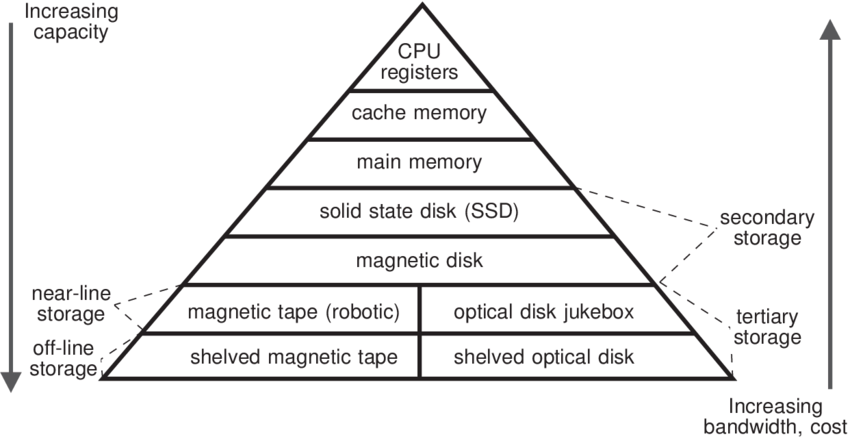
\includegraphics[width=0.7\textwidth]{storage}
    \centering
    \caption{A tárolók piramis modelle}
    \label{fig:storage}
\end{figure}

\section{Adatátvitel}
Az adatátvitel a RAM és a cache között mindig blokkos formában történik, mivel nagy valószínűséggel az utasítások és adatok felhasználása is az egymás utáni tároló címekből történik.
A processzor és a cache közötti adatátvitel ezzel szemben lehet byte szintű is.
Fontos, hogy a cache kisebb mérete miatt mindig dönteni kell, hogy a memóriából mely adatokat töltse be a rendszer.

\section{Felosztás}
A tapasztalat azt mutatta, hogy érdemes az utasításokat és az adatokat külön-külön cache-ben tárolni, ezért a modern processzorok már ezt a felépítést alkalmazzák (pl. Intel 1993-tól használ külön adat- és utasítás cache-t).
Ennek okai:
\begin{itemize}
    \item az adatok és utasítások általában elég függetlenül kezelhetők
    \item előfordulhat, hogy egy programrészlet sok adattal dolgozik (ekkor közös cache esetén előfordulhatna, hogy a sok adat miatt kikerülnek a programhoz tartozó utasítások, ami lassuláshoz vezetne)
    \item utasítás cache-nél csak az olvasást kell gyorsítani, míg adatoknál az írást és az olvasást is $\rightarrow$ eltérő technológiák
\end{itemize}
A modern, három szintű cache-t használó rendszerekben a következő típusú gyorsítótárak jelennek meg:
\begin{itemize}
    \item utasítás cache - Level 1
    \item adat cache - Level 1
    \item mixed cache - Level 2, 3
\end{itemize}

\section{Tervezési szempontok}
A cache tervezésének alapvető dilemmája, hogy el kell dönteni melyik a fontosabb: a sebesség, vagy a találti arány.
Mivel a gyorsítótárakban az adatokat keresni kell, minél nagyobb a kapacitása, annál hosszabb időbe telik a keresett adatot megtalálni.
Ezért egy olyan kompromisszumot kell kötni, amikor még nem túl sok idő megtalálni egy bizonyos adatot, de már nem kell túl gyakran az operatív tárhoz fordulni.
A processzorok gyorsulásával egyre több gyorsítótárra volt szükség, de a kapacitást már az előbb említettek miatt már nem volt hatékony növelni.
Erre a megoldás a többszintű gyorsítótár bevezetése.
Először az L1 mellett az L2, majd később az L3 cache is megjelent.
A legkisebb és leggyorsabb az L1 cache, a legnagyobb és leglassabb pedig az L3.

\section{A cache szintek összehasonlítása}
Az L1 cache a regiszter utáni leggyorsabb tároló, általában a CPU órajelén üzemel.
Mérete kicsi, nagyságrendileg 2x32 vagy 2x64 KByte.
Késleltetése alacsony, kb. 1,3-1,5 ns (3-4 óraciklus).
A késleltetések a többi cache szint között a következő táblázatban láthatóak.
\begin{center}
    \begin{tabular}{c | c | c}
        & Elérési idő (sec) & Elérés idő (ciklus) \\
        \hline
        L1 & 1,3-1,5 ns & 3-4 \\
        \hline
        L2 & 4,5-8 & 10 \\
        \hline
        L3 & 12-20 & 20-40 \\
        \hline
        RAM & 60-80 & 50-200 \\
    \end{tabular}
\end{center}

\section{Gyakorlati példák}
\begin{itemize}
    \item Intel 80486: 128 kB L1
    \item Intel P1/P2: 128 kB L1, 512 kB L2
    \item Intel P4: 256 kB L1, 1 MB L2
    \item Intel Core 2: 512 kB L1, 2-8 MB L2
    \item Intel Core i: 2x32 kB L1, 256 kB, 3-8 MB L3
\end{itemize}

\section{Memória és cache közötti kapcsolat}

\subsection{Példa a címzésre}
Egy 2 GB RAM felosztható 512 darab 4 MB-os blokkra.
A címeket kétutas asszociatív cache esetén kétfelé lehet osztani és ezeket eltárolni a blokkokban.

\subsection{Adat szinkronizáció}
Lényeges szempont a cache tároló és az operatív tár azonos részei tartalmának az egyezőségét biztosítani.
Tehát ha egy, a cache-ben tárolt operandus értéke megváltozik, azt vissza kell írni az operatív tárba is.

\subsection{Címek tárolása}
A cache-ben a memória egyes, egymást követő rekeszeinek tartalmát tároljuk, de ezek mellé el kell tárolni az adatok memóriabeli címét is.
A memória címnek csak akkora részét kell tárolni a cache-ben, amelynek alapján közvetlenül (a tárolt értékből) vagy közvetve (a tárolt értékből és annak cache-beli helyéből, sorából - cache line) a blokk kezdő címe meghatározható.
A címnek azt a részét, amelyet a cache-ben elhelyez a CPU, és ami alapján a kiválasztás történik, tagnek nevezzük.
Ez származhat fizikai vagy virtuális címből, attól függően, hogy a cache a CPU és az MMU (memory management unit), vagy az MMU és a RAM között helyezkedik el.
Az első esetben fizikai, a másodikban virtuális címekből történik a tag származtatása.
A virtuális címek használatának hátránya, hogy a tárolandó tag nagyobb, mivel a virtuális címtér is nagyobb és hosszabbak a címek.
További hátrány, hogy a virtualizációból adódó helyettesítéseket kezelni kell.
Előny ugyanakkor, hogy a virtuális tag csökkenti a cache hiba késleltetést.
A virtuális tagelés hátrányai miatt általában a mai architektúrák fizikai tageket használnak.

\subsection{Visszakeresés}
A visszakeresés módja az ún. tartalom szerinti visszakeresés (CAM - Content Address Memory), ami azt jelenti, hogy a vizsgált adatnak a cache-ben tárolt adattal való egyezőségét vizsgálja a CPU kiolvasáskor és kereséskor.
A vizsgálat a keresett adat címének összehasonlítását jelenti a cache-ben tárolt címekkel, vagy azok egy részével.
A cache akkor működik hatékonyan, ha a keresett adat a kiválasztások többségében a cache-ben, és nem a memóriában található.
Ha a keresett adat a cache-ben megtalálható, cache hitről beszélünk, ellenkező esetben cache miss lép fel.

\section{Cache hit}
A találatok aránya függ a cache
\begin{itemize}
    \item méretétől és
    \item szervezési módjától.
\end{itemize}
A modern rendszerekben a találati arány közelít a 100\%-hoz, az elvárt hibaarány 1-2\%.

\section{Cache miss}
Ha a keresett adat nem található meg a gyorsítótárban, a CPU a RAM-ból olvas, viszont a regiszeren kívül a cache-be is betölti.

\section{Replacement policy}
A cache tároló tartalmának cseréjekor a találati arány fenntartása érdekében szükséges a megfelelő helyettesítési stratégia (replacement policy) kiválasztása.
Alapértelmezés szerint a cache tele van, ezért ha más adatokra lenne szükség, mint amit jelenleg tárol, bizonyos részeit ki kell cserélni.
Ezeknek a cseréknek a módját határozza meg a replacement policy.

\section{Állapot bitek}
A cache-ben az adaton és a tagen kívül az adatok állapotára vonatkozó információt is tárolni kell.
Ezek a vezérlést és a helyettesítési eljárást kiszolgáló bitek.
A legfontosabb vezérlő bitek:
\begin{itemize}
    \item V (valid) bit
    \item D (dirty) bit
\end{itemize}

\subsection{Valid bit}
A valid bit a cache tartalmának érvényességét jelzi a cache sorra vonatkozóan.
Ha be van állítva, az adat a megadott című tárolóhelyhez tartozik, és aktuálisan érvényes.
Például törlés (flushing cache line) esetén a V bit 0-ra lesz beállítva, ezzel jelzi a processzor számára, hogy az adott területre szabadon lehet írni.
Minden blokkhoz legalább egy V bit tartozik.

\subsection{Dirty bit}
A dirty bit egy blokk valamely részének felülírását vagy módosítását jelzi.
Az ilyen blokk helyére nem lehet újat betölteni, előbb a módosított adatokat ki kell írni az operatív tárba.

\section{Jellemzők}
A cache-eket jellemző paraméterek:
\begin{itemize}
    \item méret (32kB - 20MB)
    \item elhelyezkedés (on chip - processzorlapkán, vagy off-chip - különálló)
    \item blokk méret: a fő tár és a cache között egy egységben mozgatott adatmennyiség (4-64 byte, adatnál és utasításnál eltérő lehet)
    \item sorméret (line size): az az adatmennyiség, amely egy összehasonlításnál maximálisan kijelölhető. Általában a blokk mérettel azonos, de kisebb is lehet.
    \item helyettesítési algoritmus (replacement policy): meghatározza azt a módot, ahogy a felesleges blokkot a cache-ben kiválasztjuk egy szükséges új blokk betöltésekor. Ilyen algoritmusok pl.:
    \begin{itemize}
        \item FIFO - legrégebben betöltött blokkot írja felül
        \item LIFO - legutoljára betöltött blokkot írja felül
        \item LFU (Least Frequently Used) - legritkábban használt blokkot írja felül
        \item LRO (Least Recently Used) - legrégebben használt blokkot írja felül
    \end{itemize}
    \item adat aktualizálási módszer
    \begin{itemize}
        \item write through - az adat változása esetén azonnal visszaírásra kerül az operatív tárba (biztosabb)
        \item write back - csak az adott cache line felülírása előtt aktualizál (gyorsabb, gyakrabban használt, de áramszünet esetén adatvesztés léphet fel, ezért pl. a RAID vezérlők esetében akkumulátorral támogatják a cache-t)
    \end{itemize}
    \item koherencia mechanizmus: az a módszer, amely biztosítja a fő tár és a cache tárak tartalmának egyezőségét
\end{itemize}

\section{Típusok}

\subsection{Teljesen asszociatív cache}
Egy beolvasott blokk a cache-ben bárhová (bármelyik sorba) kerülhet. Előnye a nagy találati arány és a rugalmasság, mivel mindig a legoptimálisabb adatokat tölthetjük be.
Keresésnél a CPU a tageket vizsgálja minden sorban, egyszerre, mivel az adat bárhol lehet.
Ennek megvalósításához szükséges n darab párhuzamos összehasonlító áramkör, ami viszont drága, bonyolult és nagyobb a fogyasztása.

\subsection{Direct mapping}
Ennél a megoldásnál minden memória blokk csak egy bizonyos cache line-ba tölthető be.
A blokk helyét a blokk sorszám határozza meg.
Mivel egy cache cellához több memória blokk is hozzá van rendelve, előfordulhat, hogy gyakran cserélni kell a cache tartalmát, ami teljesítmény csökkenést okozhat.
Így a megoldás rugalmatlan és kisebb a találati arány.
Előnye viszont a gyors visszakeresés és az olcsó megvalósítás (mivel csak egy összehasonlító áramkör kell).

\subsection{n-way (set) associative cache}
Az előző két módszer közötti kompromisszumot jelenti ez a módszer.
n jellemzően 2, 4, 8 vagy 16.
Az n változó meghatározza, hogy egy adott blokk hány cache line-ba kerülhet.
Például egy 4 utas asszociatív cache-nél egy blokk 4 cache line-ba kerülhet.
Eredmény, hogy a CPU a csoport index alapján 4 darab blokkra tudja szűkíteni a keresést, tehát csak 4 összehasonlító áramkör kell.
Előny, hogy rugalmasabb és nagyobb találati arányú mint a direct mapping, de olcsóbb, mint a teljesen asszociatív.
Az Intel általában 8 utas asszociatív cache-t használ.

\subsection{Sector mapping cache}
A gyakorlatban ritkán használt, itt a blokk helye kötött a csoportokon belül, viszont a csoport bárhová kerülhet.

\section{Cache hierarchia}
A gyorsítótárak hierarchiája látható a \ref{fig:hierarchia}. ábrán.
Régebbi rendszerekben csak L1 adat és utasítás cache volt, ezek fölött csak a memória állt, később megjelent az L2, majd az L3 cache is.
\begin{figure}[H]
    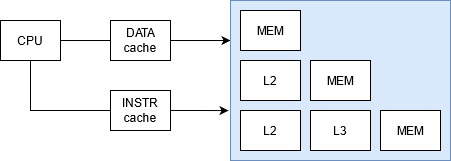
\includegraphics[width=0.7\textwidth]{hierarchia}
    \centering
    \caption{A gyorsítótárak hierachiája}
    \label{fig:hierarchia}
\end{figure}

\section{Cache line felépítése}
\paragraph{Példa:} 64 byte-os cache line esetén a cache line részei:
\begin{itemize}
    \item Directory Entry: tag és egyéb állapotjelzők.
    \item Data: maga az adat.
\end{itemize}
Ennek a felépítése látható a \ref{fig:cacheline}. ábrán.
\begin{figure}[H]
    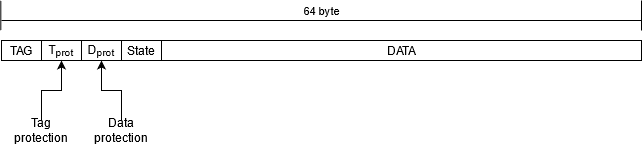
\includegraphics[width=\textwidth]{cacheline}
    \centering
    \caption{A cache line felépítése}
    \label{fig:cacheline}
\end{figure}

\section{Adat szervezési módok}
Többszintű cache-ek esetén megkülönböztetünk inclusive és exclusive gyorsítótárakat.

\subsection{Exclusive cache}
Exclusive cache esetében a tárolók egymástól függetlenek, nem tartalmazzák egymás adatait, így ugyanaz az adat nem lehet jelen egyszerre több tárban.
Az adatok betöltése kétféleképpen történhet.
Az egyik lehetőség, hogy először az L1-be töltjük be az adatokat, majd ami nem fér bele, azt az L2-be, és ami oda se, azt az L3-ba.
Ilyenkor nevezzük az L3-at victim cache-nek is.

\subsection{Inclusive cache}
Inclusive cache-eknél az L2 tartalmazza az L1 adatainak másolatát is.
Hátrány, hogy csökken L2 szabad mérete és kétszer kell írni, viszont előny, hogy L1-ben minden sor szabadon cserélhető, mert L2-ben megvan (ahonnan majd kiírásra kerülhet).
A másik előny, hogy több mag esetén, amikor egy másik mag cache-ében kell keresni az adatot, a duplikálás miatt elég L2-ben keresni.
Mivel manapság elég nagy méretű cache-eket használnak, az előnyök miatt inkább inclusive cache-t alkalmaznak (főleg több magos processzoroknál).

\section{Data prefetch logic}
További gyorsítási lehetőség a data prefetch logic, ami általában L2-ben található.
Az L1 cache adatelérési sémáit elemzi, és ha szekvenciális lekérést talál, akkor előre behúzza az adatokat a memóriából L2-be vagy L3-ba.

\section{Cache koherencia probléma}
Fontos a gyorsítótár egyezőség fenntartása több CPU vagy mag esetén.
Ezek megoldására léteznek az alábbi cache koherencia protokollok:
\begin{itemize}
    \item snoopy
    \item snorf (ritka)
    \item könyvtár alapú
    \item MESI
\end{itemize}
Cél, hogy a módosított adat a lehető leggyorsabban bekerüljön az összes processzor gyorsítótárába, mielőtt a többi esetlegesen műveletet végezne rajta.
Az adat változás érvényesítése kétféleképpen történhet:
\begin{itemize}
    \item invalidáció: érvényteleníti az összes cache tárban az adott cellát (valid bit segítségével)
    \item felülírja az új állapottal
\end{itemize}
Az első módszernél write back alapú rendszerekben előfordulhat, hogy a helyes eredmény még nem íródott vissza az operatív tárba.
Ezért nem elég invalidálni, hanem el kell kérni a helyes adatot a másik CPU-tól vagy magtól.
A felülírásos rendszernél ilyen probléma nem áll fent, a CPU vagy mag egyszerűen direktben küldi el a változott adatot a többi CPU-nak vagy magnak.
A gyakorlatban mégis inkább az invalidációt alkalmazzák, mivel egy invalidálási üzenet sokkal kisebb, mint egy teljes cache cella tartalma.

\subsection{Snoopy protokoll}
A magok vezérlői folyamatosan figyelik, "szaglásszák" a közvetítő adat buszt.
Olyan tranzakciót keresnek, amik hatással vannak önmagukra.
Például ha egy cache írási művelettel találkozik, aminek a tagje olyan, amit ő is tárol, azonnal invalidálja azt a cache line-t és elkéri az aktuális adatot a másik magtól.
Előnye az egyszerű kiépíthetőség, de hátrány, hogy terheli a buszrendszert.

\subsection{Könyvtár alapú protokoll}
A megosztott adatok egy közös könyvtárban vannak elhelyezve.
A könyvtár egy szűrőként működik, amelyen keresztül a processzornak engedélyt kell kérnie, hogy betölthessen egy adatot az operatív tárból.
Ha a bejegyzés változik, a könyvtár vagy felülírja, vagy invalidálja a többi cache tartalmát.
Ezzel a megoldással nincs szükség külön buszra.
Elsősorban NUMA rendszerekben használatos.

\subsection{MESI protokoll}
A MESI a Modified Exclusive Shared Invalid rövidítése. A protokoll állapotjelzői:
\begin{itemize}
    \item Modified: egy tár valid, a többi invalid - egyik tárban módosult de még nincs visszaírva
    \item Exclusive: érvényes adat, egyezik a fő tárral, és csak egy helyen van meg
    \item Shared: az adat a fő tárral egyezik, de több tárolóban is megtalálható
    \item Invalid: az adat érvénytelen
\end{itemize}